%tex file for ISCIE International Symposium on 
%            Stochastic Systems Theory and Its Applications
%
%

%latex209
%\documentstyle[sss,epsfig]{article}

%latex2e
\documentclass[a4paper]{article}
\usepackage{latexsym}
\usepackage{sss}
\usepackage{graphicsx} % for pdf, bitmapped graphics files
\usepackage{epsfig} % for postscript graphics files
\usepackage{amsmath}
\usepackage{here}
\usepackage{bm}

\begin{document}
\date{}
\title{\LARGE{\bf
Direction Control of Moving Vehicle using Dual RTK-GNSS and Kalman Filter}
}
\author{
Shingo Kaminokado, Jun Ogawa, Keita Nakamura, Keitaro Naruse \\
Dept. of Computer Science and Engineering, The University of Aizu\\
Turuga, Ikki-machi, Aizuwakamatsu City, Fukushima, 965-8580 \\
\\E-mail: \texttt{m5211128@u-aizu.ac.jp}
}

\maketitle
\thispagestyle{empty}
%ABSTRACT
\abstract{
We have been investing a weeding robot. The robot estimates its position with 
Global Navigation Satellite System(GNSS) but includes errors, which are around 
a few meters, when it does single positioning. The direction of the robot deviates 
a lot as it is based on location information. Hence by using the more accurate Real 
Time Kinematic GNSS (RTK-GNSS), the positional accuracy improved. However, since 
the direction of the robot was estimated from the difference with the position of 
the previous robot, it was difficult to estimate the direction while posing. Therefore, 
we presumed self-position with two single frequency RTK-GNSS receivers which become 
to be available recently and are economically friendly. By setting the normal vector
calculated from the left and right position information with two modules as 
the direction of the robot, it made it possible to estimate the direction not 
only while running but also posing. Moreover, we will tackle construction of position 
estimation system with Kalman filter.
}


\section{Introduction}
Our research group has been developed a small weeding robot\cite{aigamo}. This robot weeds automatically in paddy fields.
It is important for the robot to know the self-position because it moves in a vast environment. To know the self-position, 
some researchers use camera\cite{camera-relate} or beacon\cite{beacon-relate}. 
However, these devices easily affected by disturbance such as weather, so it is difficult to apply to our robot.
Therefore, we adopt Global Navigation Satellite System(GNSS) to obtain self-position of the robot\cite{gnss}.
Conventionally, robots obtain self-position by single-positioning method.
However, position errors and orientation errors are greatly increase.
Therefore, we adopt Real Time Kinematic-GNSS (RTK-GNSS) for higher accuracy.

GNSS modules mainly receive two kinds of carries.
Dual frequency receivers are expensive and large, so we can not mount our robot.
On the other hand, the number of satellites has increased by multi-GNSS technology in recent years. 
As a result, cheap and compact modules that can acquire one frequency carrier have been on the market.
Therefore, we adopt these modules.
We installed two modules on the both side of the robot because it is difficult to estimate the orientation of the robot using only one module\cite{rtk-gnss}\cite{auto-weeding}.
In this research, we propose a more accurate self-localization system by introducing the Kalman filter into our positioning system.
We verify our proposed method by Matlab.

\begin{figure}[H]
    \vspace{5mm}
    \centerline{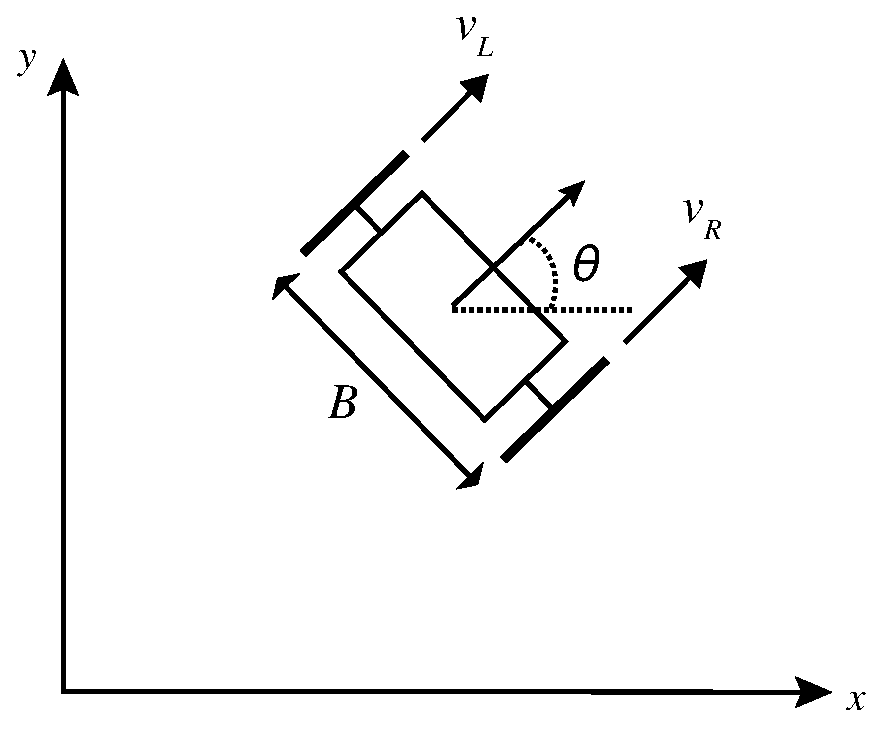
\epsfig{file=./figure/aigamo_robot_model.eps,width=50mm}}
    \caption{Robot model}
\end{figure}

\section{カルマンフィルタの説明}
この章ではカルマンフィルタの説明を行う.アイガモロボットは2次元平面上を移動する.ロボットの中心座標を$(x,y)$, $x$軸となす角を$\theta$とする.ロボットの状態ベクトル$x$は式1と表現される.
\begin{equation}
    \bm{x} = \begin{bmatrix}
        x \\
        y \\
        \theta
        \end{bmatrix} 
\end{equation}
ロボットは左右の速度$v_{L}$,$v_{R}$によって制御され,制御ベクトル$u$は式2と表現される.
\begin{equation}
    \bm{u} = \begin{bmatrix}
        v_{L} \\
        v_{R} 
        \end{bmatrix} 
\end{equation}
%
%
カルマンフィルタの一般式からロボットの推定位置は式3のように表現される
\begin{equation}
    \bm{\hat{x}}_{t} =F\bm{\hat{x}}_{t-1} + B\bm{u_{t}} + \bm{w_{t}}
\end{equation}
where, $F = \begin{bmatrix} 1 & 0 & 0 \\  0 & 1 & 0 \\  0 & 0 & 1 \end{bmatrix}$,
$B = \begin{bmatrix} dt * cos\theta & 0 \\  dt * sin\theta & 0 \\ 0 & 1 \end{bmatrix}$, 
$\bm{w}$ is process noise.\\
%
%
また,誤差共分散行列の更新は式4のように表現される
\begin{equation}
    P_{t} = F P_{t-1} F^{T} + Q
    \label{eq:4}
\end{equation}
ただし,Pは誤差共分散行列を表している. Qはプロセスの共分散行列で,\\ \\$Q = \begin{bmatrix} \sigma_{v_{L}}^{2} & 0 \\  0 & \sigma_{v_{R}}^{2} \\  \end{bmatrix}$\\ \\
%
%
GPSよるロボットの位置$z$は式5のように表現される
\begin{equation}
    \bm{z}_{t} = H\bm{x}_{t} + \bm{v}_{t}
    \label{eq:5}
\end{equation}
where,$H = \begin{bmatrix} 1 & 0 & 0 \\  0 & 1 & 0 \\  0 & 0 & 1 \end{bmatrix}$, 
$\bm{v}$ is observation noise. \\ \\
カルマンフィルタの更新フェーズでは式6−10の式で観測誤差共分散行列$S$の更新,カルマンゲイン$K$の修正,推定状態量$\bm{\hat{x}}$の更新を行う.
\begin{equation}
    \bm{y}_{t} = \bm{z}_{t} - H\bm{\hat{x}}_{t}
    \label{eq:6}
\end{equation}
%
%
\begin{equation}
    S_{t} = R + HP_{t}H^{T}
    \label{eq:7}
\end{equation}
%
%
\begin{equation}
K_{t} = P_{t}H^{T}S_{t}^{-1}
    \label{eq:8}
\end{equation}
\begin{equation}
    \bm{\hat{x}}_{t} = \bm{\hat{x}}_{t}+K_{t}\bm{y}_{t}
    \label{eq:8}
\end{equation}

\begin{equation}
    P_{t} = (I-K_{t}H^{T})P_{t}(I-K_{t}H^{T})^{T} + K_{t}RK_{t}^{T}
    \label{eq:9}
\end{equation}
%
ただし,Rは観測の共分散行列で,$R = \begin{bmatrix} \sigma_{x}^{2} & 0 & 0 \\  0 & \sigma_{y}^{2} & 0 \\  0 & 0 & \sigma_{\theta}^{2} \end{bmatrix}$\\



\section{Pre experiments}
%Experiments on acquisition of covariance matrix for Kalman filter
%先行研究においてカルマンフィルタに用いる誤差分布を調査した.
We investigated the error distribution used for the Kalman filter in the previous study.
\subsection{Experimental device}
%RTK-GNSSには,最低でも基地局と移動局の2つGNSSモジュールが必要だが,
%本実験では,基地局にEmlid社のReach RS[2]を1台と移動局にEmlid社のReach[3]を2台用いる.
%基準局は図1に示すように,見晴らしの良い四等三角点の地上高1.5m地点に設置する.
%移動局は,GNSSモジュールをロボットの左右に設置することを想定して,
%図2に示すような実験装置を用いる.基準局と移動局のアンテナの下には,
%地面からのマルチパスを防ぐため10cm×10cmのアルミプレートを敷く.
RTK-GNSS requires at least GNSS modules, base station and rover. 
In this experiment, we use one Reach RS\cite{reach rs} from Emlid as a base station 
and two Reach\cite{reach} from Emlid as a rover.
As shown in Figure 2, the base station is installed at a position of 1.5m above the ground 
with a quaint triangle with a clear view.
Rover uses an experimental apparatus as shown in Figure 3. 
Under the antennas of the base station and the mobile station, 
an aluminum plate of 10 cm x 10 cm is laid down to prevent multipass from the ground.

\begin{figure}[H]
    \centerline{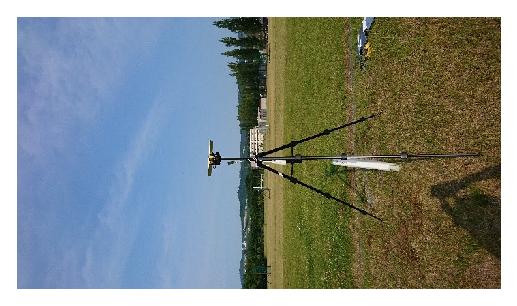
\epsfig{file=./figure/fig1.eps,width=50mm,angle=-90}}
    \caption{Base Environment}
\end{figure}
\begin{figure}[H]
    \centerline{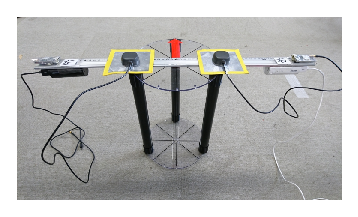
\epsfig{file=./figure/fig2.eps,width=50mm}}
    \caption{Rover}
\end{figure}

\subsection{Investigation method}
%先行研究では,移動局に2つのモジュールを用いた場合の位置誤差,向きの誤差,
%モジュール間距離の影響,方位による影響を調べるために以下のデータセットを測定した.
%それぞれのデータセットは周波数5Hzで20秒間(100データ)を45度刻みに8方位取得する.
In the previous study, the following data set was measured in order to 
investigate the position error, the orientation error, 
the influence of the module distance and orientation, when two modules were used for a rover.
Each data set acquires 8 azimuths at a frequency of 5 Hz (100 data) in increments of 45 degrees.
\begin{enumerate}
    \renewcommand{\labelenumi}{(\roman{enumi})}
    \item Ground height 30cm/Distance between modules 20cm
    \item Ground height 30cm/Distance between modules 30cm
    \item Ground height 30cm/Distance between modules 40cm
    \item Ground height 150cm/Distance between modules 20cm
    \item Ground height 150cm/Distance between modules 30cm
    \item Ground height 150cm/Distance between modules 40cm
\end{enumerate}

\subsection{Result}
%一番実環境に近い(ⅱ)の結果を図4と5に示す.
Figures 4 and 5 show the results of (ii) which is closest to the real environment.

\begin{figure}[H]
    \centerline{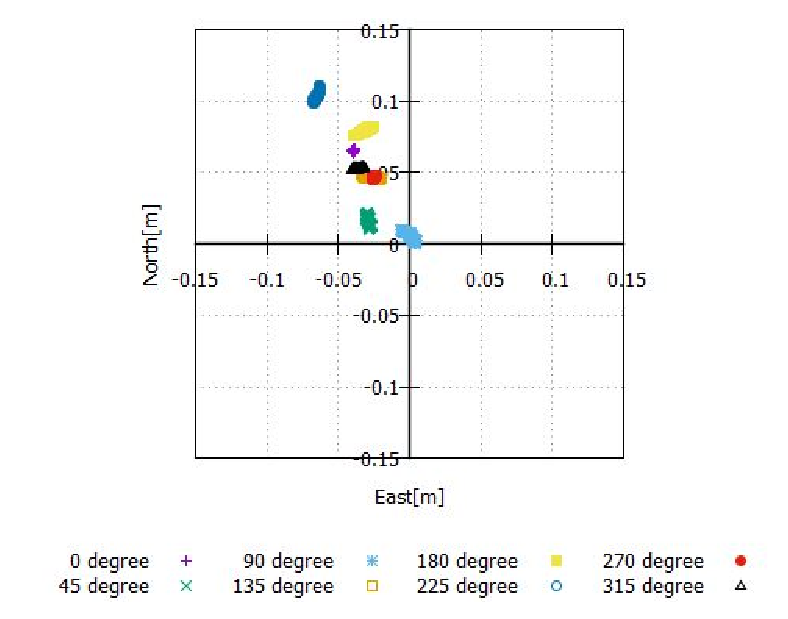
\epsfig{file=./figure/30dis_30hight.eps,width=70mm}}
    \caption{Position error}
\end{figure}
\begin{figure}[H]
    \centerline{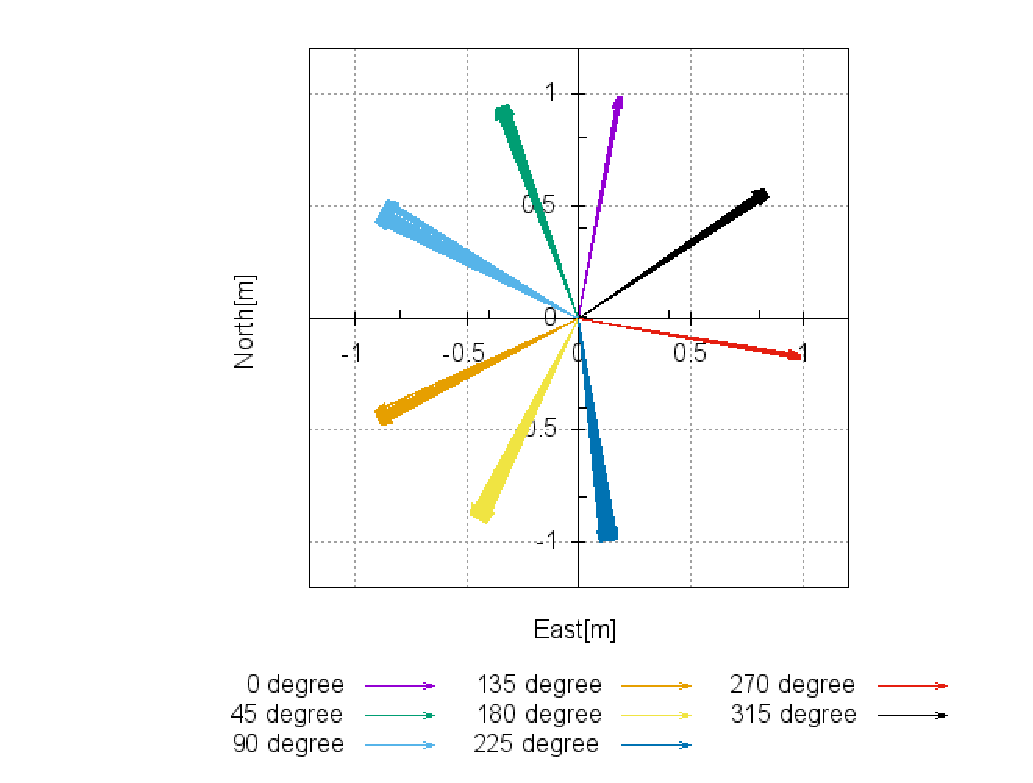
\epsfig{file=./figure/30dis_30hight_vector.eps,width=70mm}}
    \caption{Orientation variation}
\end{figure}

%これより得られた誤差データより分散共分散行列を算出する.
%位置のみの多変量正規分布を図6に示す
A variance covariance matrix is ​​calculated from the error data obtained from this experiment. 
The multivariate normal distribution of only the position is shown in figure 6.
\begin{figure}[H]
    \centerline{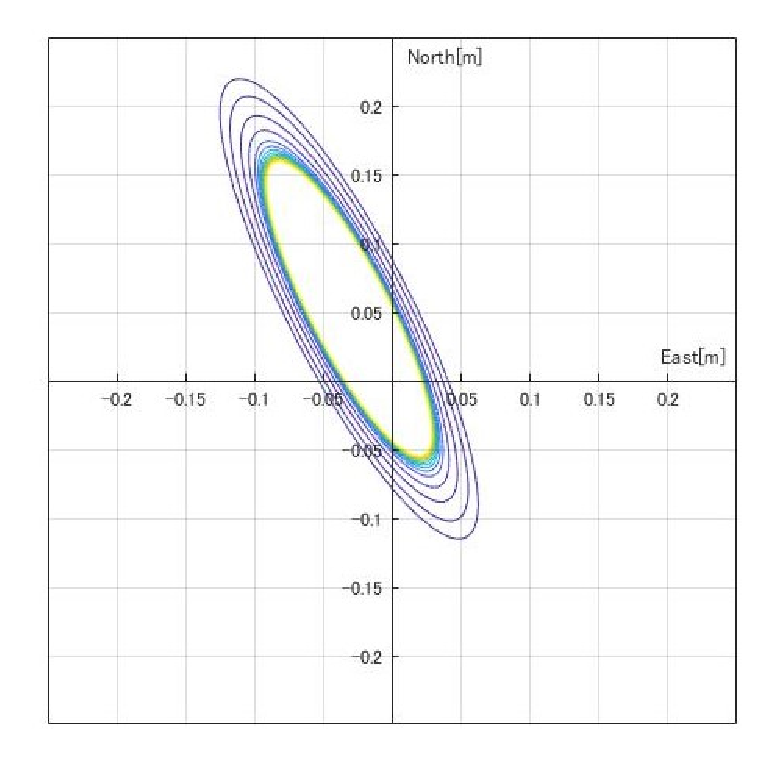
\epsfig{file=./figure/fig13.eps,width=70mm}}
    \caption{Multivariate normal distribution}
\end{figure}

%ロボットの向きも加えた平均と分散共分散行列を式10,11に示す.
The mean and variance covariance matrix with the orientation of the robot 
also added are shown in equations 10 and 11.

\begin{equation}
    \begin{split}
     \mu = 
     \begin{bmatrix}
        \mu_x \\
        \mu_y \\
        \mu_\theta
     \end{bmatrix}
     =
     \begin{bmatrix}
        0.0523096875 \\
        -0.0315079375 \\
        -0.0287904375
     \end{bmatrix}
    \end{split}
    \label{eq:10} 
\end{equation}

\begin{equation}
    R = 
    \begin{bmatrix}
        0.0000041093 & -0.0000001684 & -0.0000053749 \\
        -0.0000001684 & 0.0000058535 & 0.0000322863 \\
        -0.0000053749 & 0.0000322863 & 0.0003444646 
    \end{bmatrix}
    \label{eq:11} 
\end{equation}

\section{Simulation using Kalman filter}
%先行研究より、我々の測位システムの位置と向きの分散共分散行列を算出した.
%式(10),(11)用いてDual RTK-GNSSにおけるカルマンフィルタの優位性についてシミュレーションする.
%シミュレーションに用いる各パラメータは表1に示す.
%ロボットは反時計周りのシーケンス制御をする.
%路面状況を考慮して車輪には大中小のノイズを与える.
%アイガモロボットの走行する路面は不整地の水田なのでノイズ大を想定している.

From the previous experiment, the variance covariance matrix of the position and orientation 
of our positioning system was calculated. We simulate the superiority of the Kalman filter 
in Dual RTK-GNSS by using equations 10 and 11. The parameters used in the simulation 
are shown in Table 1. The robot performs sequence control in the counterclockwise 
direction. In consideration of the road surface condition, we give large, medium and small noise 
to the wheels. Since the road surface on which the Aigamo robot runs is an irregular 
rice field, it assumes a large noise.


\begin{table}[H]
    \caption{Parameters for simulation}
    \label{table:table1}
    \centering
    \begin{tabular}{|l|l|}
        \hline
        Parameter & Value \\
        \hline \hline
        Wheel distance \(B\) & \(0.35[m]\) \\
        Left wheel speed \(v_L\) & \(0.2 [m/s]\) \\
        Right wheel speed \(v_R\) & \(0.3 [m/s]\) \\
        Robot control frequency & \(100 [Hz]\) \\
        Update frequency of GNSS & \(5 [Hz]\) \\
       \hline
    \end{tabular}
\end{table}

\newlength{\myheight}
\setlength{\myheight}{1.2cm}

\begin{table}[h]
    \caption{Wheel noise}
    \label{table:table2}
    \centering
    
    \begin{tabular}{|l|l|}
    \hline
    Magnitude of noise & Convariance matrix \\
    \hline \hline
    \parbox[c][\myheight][c]{0cm}{} small & $ Q =  
        \begin{bmatrix}
            0.1^2 &0 \\
            0     &0.1^2 \\ 
        \end{bmatrix}
        $ \\
    \hline
    \parbox[c][\myheight][c]{0cm}{} middle & $ Q =  
    \begin{bmatrix}
            0.3^2 &0 \\
            0     &0.3^2 \\ 
        \end{bmatrix}
        $ \\
    \hline
    \parbox[c][\myheight][c]{0cm}{} large & $ Q =  
        \begin{bmatrix}
            1^2 &0 \\
            0     &1^2 \\ 
        \end{bmatrix}
        $ \\
    \hline
    \end{tabular}
\end{table}

\subsection{Result}
%車輪外乱大中小の時のシミュレーション結果をFiure 1~3に示した.
%
%

The simulation results for large, medium and small wheels 
disturbance are shown in Figure 7 to 9.

\begin{figure}[H]
\centerline{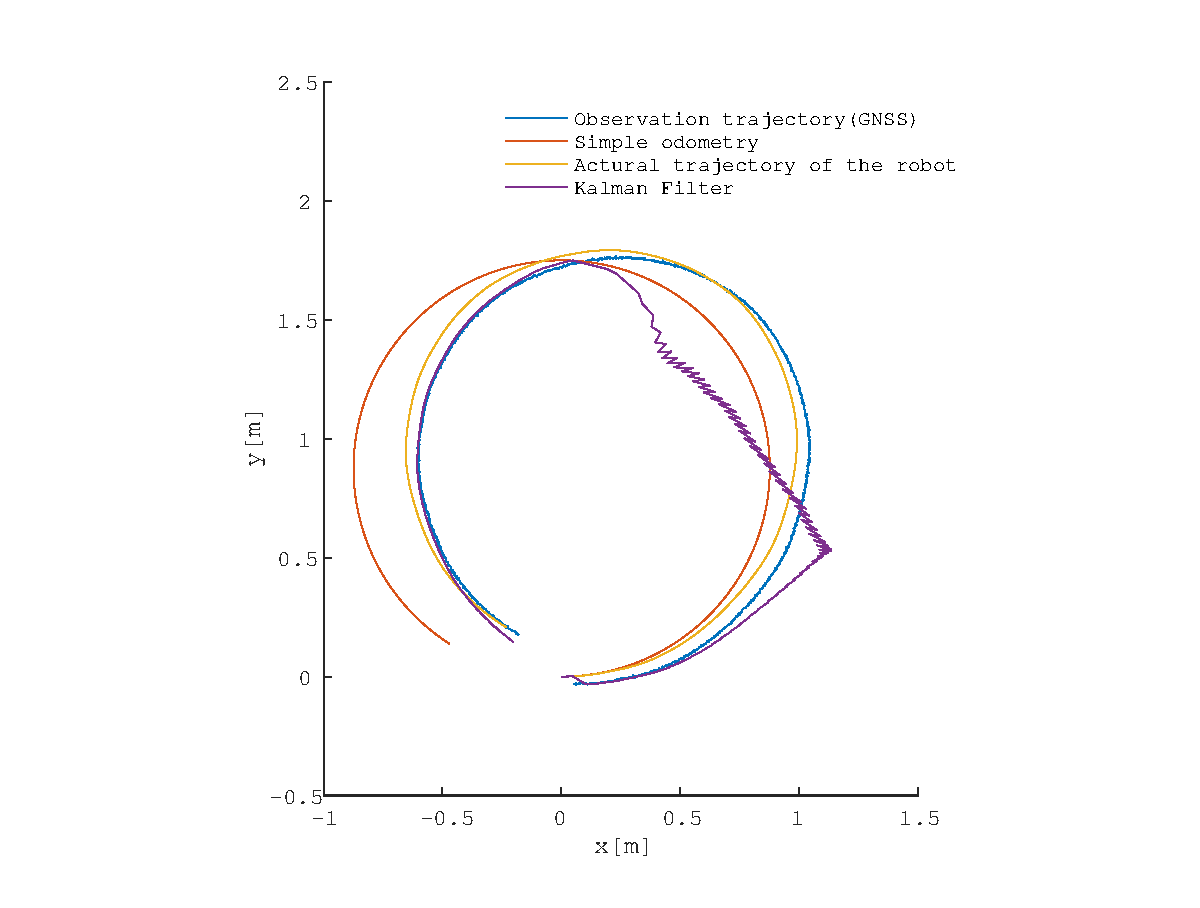
\epsfig{file=./figure/process_noise_S.eps,width=100mm}}
\caption{Small process noise}
\end{figure}
\begin{figure}[H]
\centerline{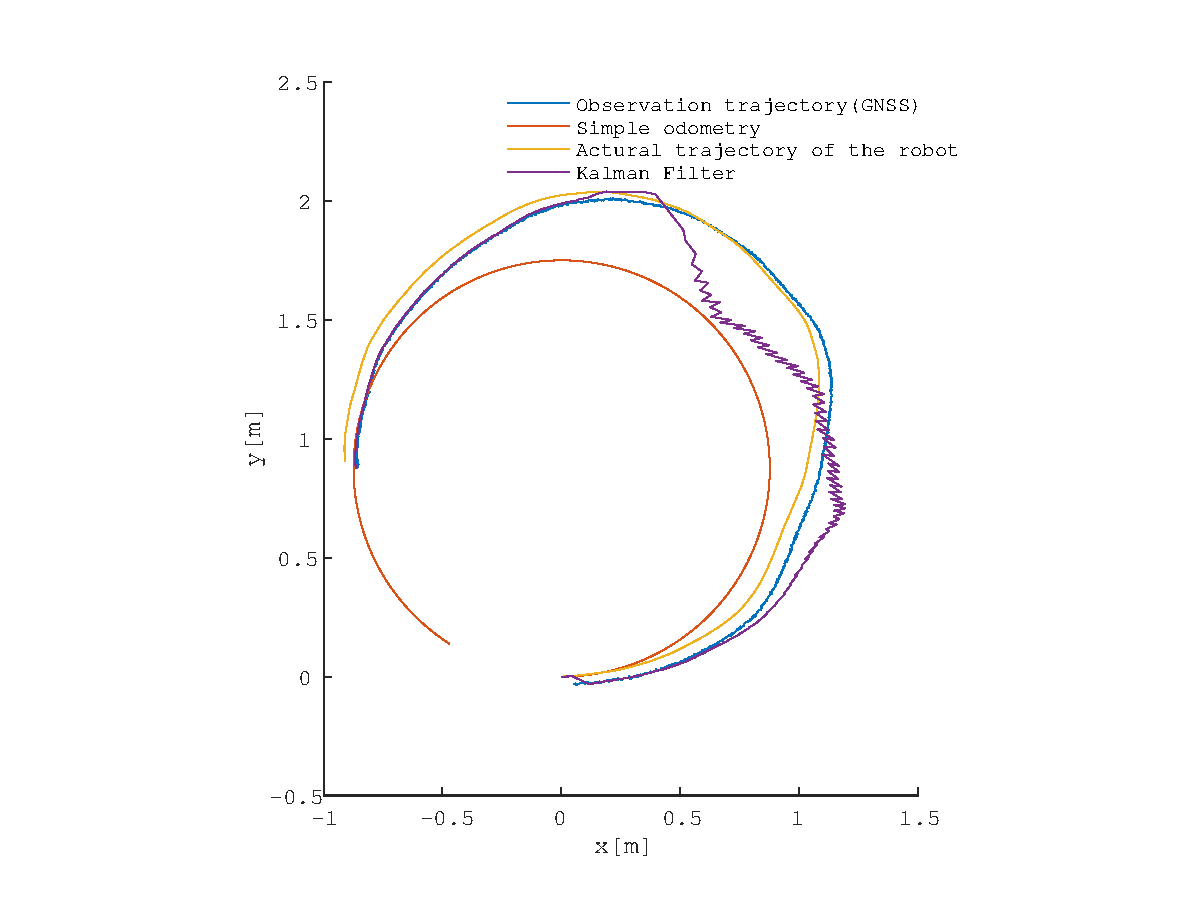
\epsfig{file=./figure/process_noise_M.eps,width=100mm}}
\caption{Middle process noise}
\end{figure}
\begin{figure}[H]
\centerline{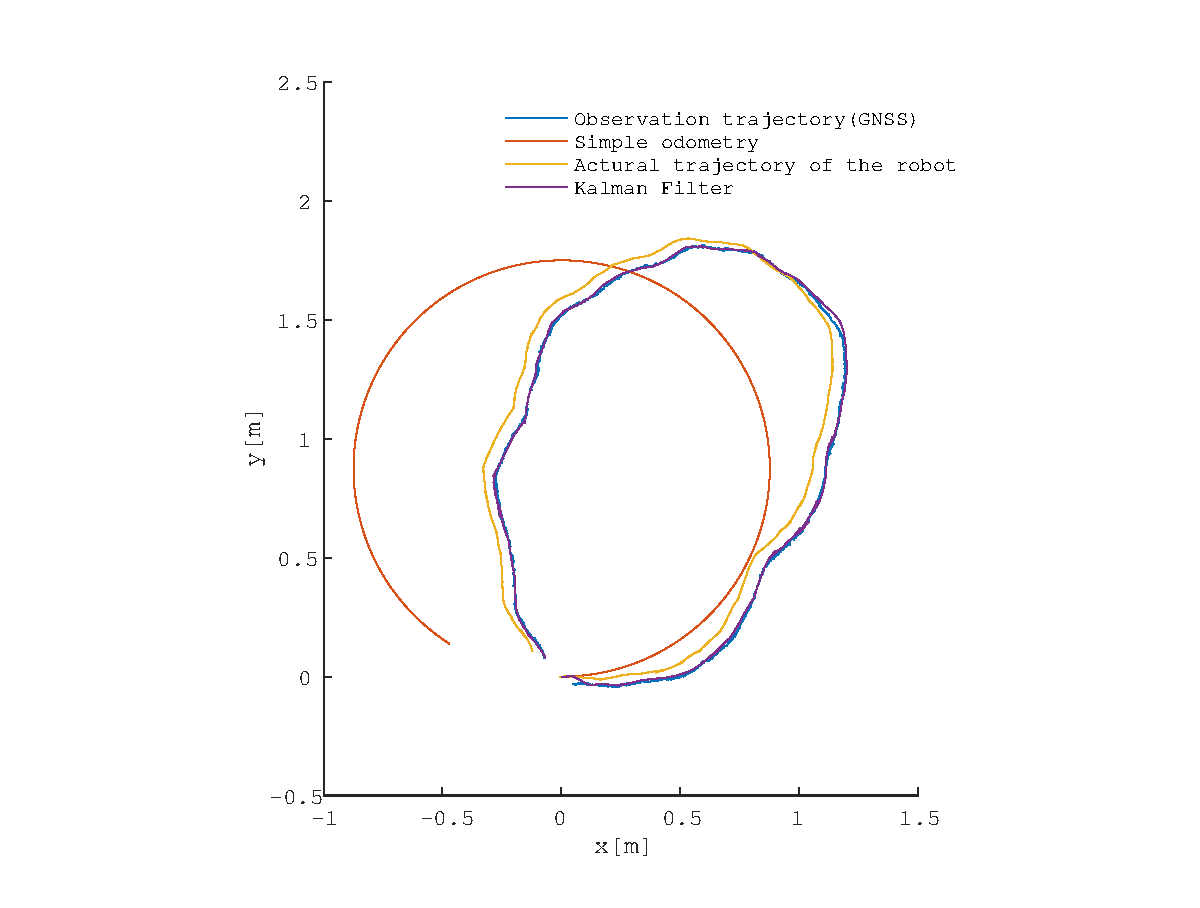
\epsfig{file=./figure/process_noise_L.eps,width=100mm}}
\caption{Large process noise}
\end{figure}
\subsection{Disucussion}
%
%
%
%
%

\section{Conclusions}
%
%
%
%
%
%

\begin{thebibliography}{99}
\bibitem{aigamo}
M. Taku, O. Yoshiaki, O. Jun, N. Keita and N. Keitaro:
Mechanism of generating drawbar pull of rod wheel on loose soil,
{\it 22rd International Symposium on Artificial Life and Robotics.(AROB)}, Vol.22, No.4, 2017.
\bibitem{camera-relate}
S.Shotaro, H. Zhencheng and F. Thomas:
Tracking ofFeatUre PointsforVisualSLAM with MultipleCameras
{\it The Institude of Image Information and Television Engineers}
\bibitem{beacon-relate}
Z. Fang, L. Deng, Y. Ou and X. Wu:
A tracking robot based on wireless beacon
{\it International Conference on Intelligent Robotics and Applications}, pp.191-202, 2010.
\bibitem{gnss}
H. J. Christopher and C. Eric:
Evolution of the global navigation satellitesystem (gnss),
{\it Proceedings of the IEEE}, Vol.96, No.12, pp.1902-1917, 2008.
\bibitem{rtk-gnss}
K. Michio. N. Noboru, I. Kazunobu and T. Hideo: 
Field Mobile Robot navigated by RTK-GPS and FOG, 
{\it Journal of the Japanese Society of Agricultural Machinery}, Vol.63, No.5, pp.74-79, 2001.(in Japanese)
\bibitem{auto-weeding}
S. Masahiro, N. Yoshisada, T. Katsuhiko and K. Kyou: 
{\it Journal of the Japanese Society of Agricultural Machinery}, Vol.72, No.3, pp.276-282, 2010.(in Japanese)
\bibitem{reach rs} 
Emlid Reach RS, https://docs.emlid.com/eachrs/

\bibitem{reach} 
Emlid Reach, https://docs.emlid.com/each/
\end{thebibliography}
\end{document}

% end of sss10.tex
